\documentclass[a4paper,12pt]{article}
\usepackage[left=3cm, right=2.5cm, top=2.5cm, bottom=2.5cm]{geometry}
\usepackage{graphicx}
\usepackage{longtable}
\usepackage{booktabs}
\usepackage{amssymb} % For the checkmark symbol
\usepackage{multirow}
\usepackage{array}
\usepackage{titlesec}
\usepackage{float} % Added for better table positioning

% Adjust section formatting
\titleformat{\section}
  {\normalfont\Large\bfseries}{\thesection.}{1em}{}

\begin{document}

% -------------------------------------------------------------------
% TITLE PAGE
% -------------------------------------------------------------------
\begin{titlepage}
    \centering
    \vspace*{1cm}
    
    % Logos
    
    {\Large \textbf{RENCANA PEMBELAJARAN DAN KEGIATAN MAGANG}} \\
    \vspace{0.5cm}
    {\Large \textbf{MERDEKA BELAJAR KAMPUS MERDEKA (MBKM)}} \\
    \vspace{0.5cm}
    {\large \textbf{SOFTWARE ENGINEERING DIVISION - PT SUMBER CIPTA MULTINIAGA}}
    
    \vspace{2cm}
    \begin{minipage}{0.49\textwidth}
        \centering
        % [Logo UGM]
        
\includegraphics[width=5cm]{gambar/logo-ugm.png} % Replace with actual file
    \end{minipage}
    \hfill
    \begin{minipage}{0.49\textwidth}
        \centering
        % [Logo Kaskus / PT Sumber Cipta Multiniaga]
        
\includegraphics[width=5cm]{gambar/logo-scm.png} % Replace with actual file
    \end{minipage}
    
    \vspace{2cm}

    Disusun oleh: \\
    \vspace{0.5cm}
    {\large \textbf{Muhammad Argya Vityasy}} \\
    \textbf{NIM: 23/522547/PA/22475}
    
    \vspace{1.5cm}
    
    Periode Semester 6 Tahun Akademik 2024/2025
    
    \vspace{2cm}
    
    \textbf{PROGRAM STUDI S1 ILMU KOMPUTER} \\
    \textbf{FAKULTAS MATEMATIKA DAN ILMU PENGETAHUAN ALAM} \\
    \textbf{UNIVERSITAS GADJAH MADA} \\
    \textbf{YOGYAKARTA} \\
    \textbf{2026}
    
\end{titlepage}

% -------------------------------------------------------------------
% SECTION 1: PENDAHULUAN
% -------------------------------------------------------------------
\section{Pendahuluan}
Dokumen ini menguraikan rencana kegiatan magang dan pembelajaran yang dilaksanakan secara hybrid di PT Sumber Cipta Multiniaga (GDP Labs) selama periode semester 5 hingga 6, sebagai implementasi program Merdeka Belajar Kampus Merdeka (MBKM). Kegiatan ini bertujuan untuk memberikan pengalaman industri yang relevan dalam program studi ilmu komputer, khususnya dalam pengembangan platform komunitas berskala besar, serta mengasah kompetensi teknis dan kolaborasi tim.

Guna memenuhi persyaratan konversi SKS, terlampir daftar mata kuliah semester 1 sampai 5 yang telah diselesaikan sesuai standar kelulusan sebagai bukti pemenuhan kewajiban akademik.

% -------------------------------------------------------------------
% SECTION 2: CHECKLIST MATA KULIAH
% -------------------------------------------------------------------
\section{Checklist Mata Kuliah Semester 1-5}

\begin{longtable}{|c|c|l|p{6.5cm}|c|c|c|}
    \hline
    \textbf{Sem} & \textbf{No} & \textbf{Kode MK} & \textbf{Nama MK} & \textbf{SKS} & \textbf{Jenis} & \textbf{Status} \\
    \hline
    \endfirsthead
    \hline
    \textbf{Sem} & \textbf{No} & \textbf{Kode MK} & \textbf{Nama MK} & \textbf{SKS} & \textbf{Jenis} & \textbf{Status} \\
    \hline
    \endhead
    
    % SEMESTER 1
    \multirow{9}{*}{1} 
    & 1 & MII211201 & Pemrograman & 3 & Wajib & $\checkmark$ \\
    & 2 & MII211202 & Praktikum Pemrograman & 1 & Wajib & $\checkmark$ \\
    & 3 & MII211002 & Logika Informatika & 2 & Wajib & $\checkmark$ \\
    & 4 & MII211001 & Aljabar Linier Fundamental & 2 & Wajib & $\checkmark$ \\
    & 5 & MMM1101 & Kalkulus 1 & 3 & Wajib & $\checkmark$ \\
    & 6 & MKK1101 & Kimia Dasar 1 & 3 & Wajib & $\checkmark$ \\
    & 7 & MFF1011 & Fisika Dasar 1 & 3 & Wajib & $\checkmark$ \\
    & 8 & UNU222013 & Bahasa Indonesia & 2 & Wajib & $\checkmark$ \\
    & 9 & UNU222005 & Agama Islam & 2 & Wajib & $\checkmark$ \\
    \hline
    \multicolumn{4}{|r|}{\textbf{Jumlah SKS Semester}} & \textbf{21} & & $\checkmark$ \\
    \multicolumn{4}{|r|}{\textbf{Jumlah SKS Kumulatif}} & \textbf{21} & & $\checkmark$ \\
    \hline
    
    % SEMESTER 2
    \multirow{10}{*}{2} 
    & 1 & MII211203 & Algoritma dan Struktur Data & 3 & Wajib & $\checkmark$ \\
    & 2 & MII211004 & Bahasa Inggris & 2 & Wajib & $\checkmark$ \\
    & 3 & MII211005 & Integral dan Persamaan Differensial & 3 & Wajib & $\checkmark$ \\
    & 4 & MII211006 & Matematika Diskrit & 3 & Wajib & $\checkmark$ \\
    & 5 & MII211601 & Organisasi dan Arsitektur Komputer & 2 & Wajib & $\checkmark$ \\
    & 6 & MII211007 & Pengantar Statistika & 2 & Wajib & $\checkmark$ \\
    & 7 & MII211204 & Praktikum Algoritma dan Struktur Data & 1 & Wajib & $\checkmark$ \\
    & 8 & MII211602 & Sistem Digital & 2 & Wajib & $\checkmark$ \\
    & 9 & UNU222011 & Pancasila & 2 & Wajib & $\checkmark$ \\
    & 10 & UNU222012 & Kewarganegaraan & 2 & Wajib & $\checkmark$ \\
    \hline
    \multicolumn{4}{|r|}{\textbf{Jumlah SKS Semester}} & \textbf{22} & & $\checkmark$ \\
    \multicolumn{4}{|r|}{\textbf{Jumlah SKS Kumulatif}} & \textbf{43} & & $\checkmark$ \\
    \hline

    % SEMESTER 3
    \multirow{10}{*}{3} 
    & 1 & MII212201 & Analisis Algoritma dan Kompleksitas & 3 & Wajib & $\checkmark$ \\
    & 2 & MII212501 & Basis Data & 3 & Wajib & $\checkmark$ \\
    & 3 & MII212601 & Jaringan Komputer & 2 & Wajib & $\checkmark$ \\
    & 4 & MII212401 & Kecerdasan Artifisial & 3 & Wajib & $\checkmark$ \\
    & 5 & MII212010 & Penulisan Akademik dan Etika & 2 & Wajib & $\checkmark$ \\
    & 6 & MII212502 & Praktikum Basis Data & 1 & Wajib & $\checkmark$ \\
    & 7 & MII212603 & Praktikum Sistem Komputer dan Jaringan & 1 & Wajib & $\checkmark$ \\
    & 8 & MII212001 & Probabilitas dan Proses Stokastika & 2 & Wajib & $\checkmark$ \\
    & 9 & MII212602 & Sistem Operasi & 2 & Wajib & $\checkmark$ \\
    & 10 & MII213208 & Computational Thinking & 2 & Pilihan & $\checkmark$ \\
    & 11 & MII212204 & Pengolahan Citra Digital & 3 & Pilihan & $\checkmark$ \\
    \hline
    \multicolumn{4}{|r|}{\textbf{Jumlah SKS Semester}} & \textbf{24} & & $\checkmark$ \\
    \multicolumn{4}{|r|}{\textbf{Jumlah SKS Kumulatif}} & \textbf{67} & & $\checkmark$ \\
    \hline

    % SEMESTER 4
    \multirow{9}{*}{4} 
    & 1 & MII212503 & Metode Rekayasa Perangkat Lunak & 2 & Wajib & $\checkmark$ \\
    & 2 & MII212504 & Workshop Implementasi RPL & 2 & Wajib & $\checkmark$ \\
    & 3 & MII212402 & Pembelajaran Mesin & 3 & Wajib & $\checkmark$ \\
    & 4 & MII212202 & Bahasa dan Automata & 3 & Wajib & $\checkmark$ \\
    & 5 & MII212203 & Metode Numerik & 2 & Wajib & $\checkmark$ \\
    & 6 & MII212209 & Kriptografi dan Keamanan Informasi & 3 & Wajib & $\checkmark$ \\
    & 7 & MII212003 & Pengembangan Startup Digital & 2 & Wajib & $\checkmark$ \\
    & 8 & MII212610 & Komputasi Awan & 3 & Pilihan & $\checkmark$ \\
    & 9 & MII212506 & Pengembangan Perangkat Lunak Scalable & 3 & Pilihan & $\checkmark$ \\
    \hline
    \multicolumn{4}{|r|}{\textbf{Jumlah SKS Semester}} & \textbf{23} & & $\checkmark$ \\
    \multicolumn{4}{|r|}{\textbf{Jumlah SKS Kumulatif}} & \textbf{90} & & $\checkmark$ \\
    \hline

    % SEMESTER 5
    \multirow{8}{*}{5} 
    & 1 & MII213401 & Pembelajaran Mesin Mendalam & 3 & Wajib & $\checkmark$ \\
    & 2 & MII213501 & Proyek Rekayasa Perangkat Lunak & 3 & Wajib & $\checkmark$ \\
    & 3 & MII213002 & Metodologi Penelitian Ilmu Komputer & 2 & Wajib & $\checkmark$ \\
    & 4 & MII213602 & Keamanan Sistem dan Siber & 3 & Pilihan & $\checkmark$ \\
    & 5 & MII213201 & Metode Optimasi & 3 & Pilihan & $\checkmark$ \\
    & 6 & MII213502 & Web Semantik & 3 & Pilihan & $\checkmark$ \\
    & 7 & MII213601 & Arsitektur dan Infrastruktur Berkinerja Tinggi & 3 & Pilihan & $\checkmark$ \\
    & 8 & MII213504 & Pengantar Penjaminan Kualitas Perangkat Lunak & 3 & Pilihan & $\checkmark$ \\
    \hline
    \multicolumn{4}{|r|}{\textbf{Jumlah SKS Semester}} & \textbf{23} & & $\checkmark$ \\
    \multicolumn{4}{|r|}{\textbf{Jumlah SKS Kumulatif}} & \textbf{113} & & $\checkmark$ \\
    \hline
\end{longtable}

% -------------------------------------------------------------------
% SECTION 3: RENCANA MATA KULIAH
% -------------------------------------------------------------------
\section{Rencana Mata Kuliah Semester 6 (MBKM)}

Berikut adalah rencana mata kuliah dan pilihan kegiatan MBKM yang diajukan untuk Semester 6:

\begin{table}[H] % Changed to [H] or just remove formatting and let it float, but here we keep it tight
    \centering
    \begin{tabular}{|c|c|p{7cm}|c|c|c|}
        \hline
        \textbf{No} & \textbf{Kode MK} & \textbf{Nama MK/Kegiatan} & \textbf{SKS} & \textbf{Jenis} & \textbf{Status} \\
        \hline
        1 & MII21-4001 & Proposal Skripsi & 2 & Wajib & Rencana \\
        2 & UNU24-2033 & Literasi Kesehatan & 2 & Wajib & Rencana \\
        \hline
        \multicolumn{3}{|r|}{\textbf{Jumlah SKS MK Wajib Prodi}} & \textbf{4} & & \\
        \hline
        3 & MII21-3011 & Internship: Pengembangan Fitur dan Modul Proyek & 4 & Pilihan & Rencana \\
        4 & MII21-3013 & Internship: Implementasi Prototipe Produk & 4 & Pilihan & Rencana \\
        5 & MII21-3014 & Internship: Pengembangan Backend & 4 & Pilihan & Rencana \\
        6 & MII21-3015 & Internship: Pengujian Unit dan Modul Proyek & 3 & Pilihan & Rencana \\
        7 & MII21-3016 & Internship: Pengujian Integrasi dan Sistem & 3 & Pilihan & Rencana \\
        8 & MII21-4012 & Soft skill: Kemampuan Bekerjasama dan Kolaborasi & 2 & Pilihan & Rencana \\
        \hline
        \multicolumn{3}{|r|}{\textbf{Jumlah SKS Kegiatan MBKM}} & \textbf{20} & & \\
        \hline
        \multicolumn{3}{|r|}{\textbf{Jumlah SKS Total Semester 6}} & \textbf{24} & & \\
        \hline
    \end{tabular}
\end{table}

% Use clearpage to force the table to print before starting the next section
\clearpage

% -------------------------------------------------------------------
% SECTION 4: DESKRIPSI KEGIATAN
% -------------------------------------------------------------------
\section{Deskripsi Kegiatan di PT Sumber Cipta Multiniaga dan Relevansi MBKM}

Kegiatan magang yang saya laksanakan di PT Sumber Cipta Multiniaga (GDP Labs) berfokus pada pengembangan sistem \textit{Digital Employee (DE)}, yaitu sebuah platform \textit{AI automation agent} yang digunakan oleh berbagai stakeholder seperti HR, Product Manager, dan tenant untuk mengotomatisasi alur kerja bisnis. Sistem ini berjalan di dalam \textit{AI runtime environment} dan terintegrasi dengan \textit{Model Context Protocol (MCP)} untuk mendukung orkestrasi tools dan eksekusi agent secara modular.

Selain itu, saya juga berkontribusi dalam pengembangan \textit{Identity and Access Management (IAM) SDK}, yaitu library terpusat untuk menangani autentikasi dan otorisasi antar layanan, sehingga mengurangi duplikasi implementasi (\textit{reinventing the wheel}) pada berbagai aplikasi internal.

Berikut adalah pemetaan kegiatan terhadap mata kuliah MBKM yang diajukan:

\subsection*{1. Internship: Pengembangan Fitur dan Modul Proyek (4 SKS)}
Saya mengembangkan fitur-fitur inti pada sistem Digital Employee secara end-to-end, mulai dari perancangan hingga implementasi. Fitur yang dikembangkan mencakup integrasi agent dengan berbagai tools melalui MCP, serta pengembangan modul automasi untuk mendukung use-case bisnis seperti reporting dan escalation handling. Pengembangan dilakukan dengan prinsip \textit{clean code} dan \textit{modular design} agar mudah di-maintain dan scalable.

\subsection*{2. Internship: Implementasi Prototipe Produk (4 SKS)}
Saya membangun \textit{proof-of-concept} (PoC) untuk berbagai skenario penggunaan AI agent dalam Digital Employee, termasuk validasi integrasi dengan AI runtime environment dan orkestrasi multi-tools. Prototipe ini digunakan untuk menguji kelayakan teknis sebelum diintegrasikan ke sistem produksi.

\subsection*{3. Internship: Pengembangan Backend (4 SKS)}
Saya berfokus pada pengembangan sisi backend menggunakan Python, termasuk membangun API, mengelola komunikasi antar service, serta mengintegrasikan IAM SDK untuk autentikasi dan otorisasi berbasis token. Selain itu, saya juga mengembangkan IAM SDK dengan pendekatan \textit{clean architecture} untuk memastikan fleksibilitas dan reusability pada berbagai sistem.

\subsection*{4. Internship: Pengujian Unit dan Modul Proyek (3 SKS)}
Saya bertanggung jawab untuk memastikan kualitas kode melalui penulisan \textit{unit test} dan \textit{integration test} dengan target \textit{100\% test coverage}. Pengujian dilakukan untuk seluruh modul yang dikembangkan, termasuk validasi alur autentikasi IAM dan eksekusi agent. Pendekatan ini bertujuan untuk meminimalkan bug pada lingkungan produksi dan meningkatkan reliability sistem.

\subsection*{5. Internship: Pengujian Integrasi dan Sistem (3 SKS)}
Saya melakukan pengujian integrasi antar komponen sistem, termasuk interaksi antara AI agent, MCP, dan layanan eksternal. Pengujian ini memastikan bahwa seluruh sistem dapat berjalan secara end-to-end dalam environment produksi, serta mampu menangani skenario kegagalan (\textit{failure handling}) dengan baik.

\subsection*{6. Soft Skill: Kemampuan Bekerjasama dan Kolaborasi (2 SKS)}
Saya bekerja dalam tim menggunakan metodologi Agile/Scrum, dengan aktivitas rutin seperti \textit{daily stand-up}, \textit{sprint planning}, dan \textit{code review}. Workflow pengembangan menggunakan Git dan GitHub, termasuk branching strategy, pull request, dan collaborative debugging. Kolaborasi dilakukan secara intensif dengan sesama engineer, Product Manager, dan QA untuk memastikan kualitas dan ketepatan waktu delivery.

\section{Penutup}
Dengan pengajuan ini, saya berharap kegiatan magang di PT Sumber Cipta Multiniaga dapat dikonversi sebagai bagian dari program MBKM. Pengalaman ini memberikan pemahaman mendalam terkait pengembangan sistem berbasis AI, arsitektur backend, serta praktik rekayasa perangkat lunak di lingkungan industri.

% -------------------------------------------------------------------
% LAMPIRAN
% -------------------------------------------------------------------
\newpage
\section*{Lampiran}

\subsection*{i. Letter of Acceptance (LoA)}
\begin{center}
    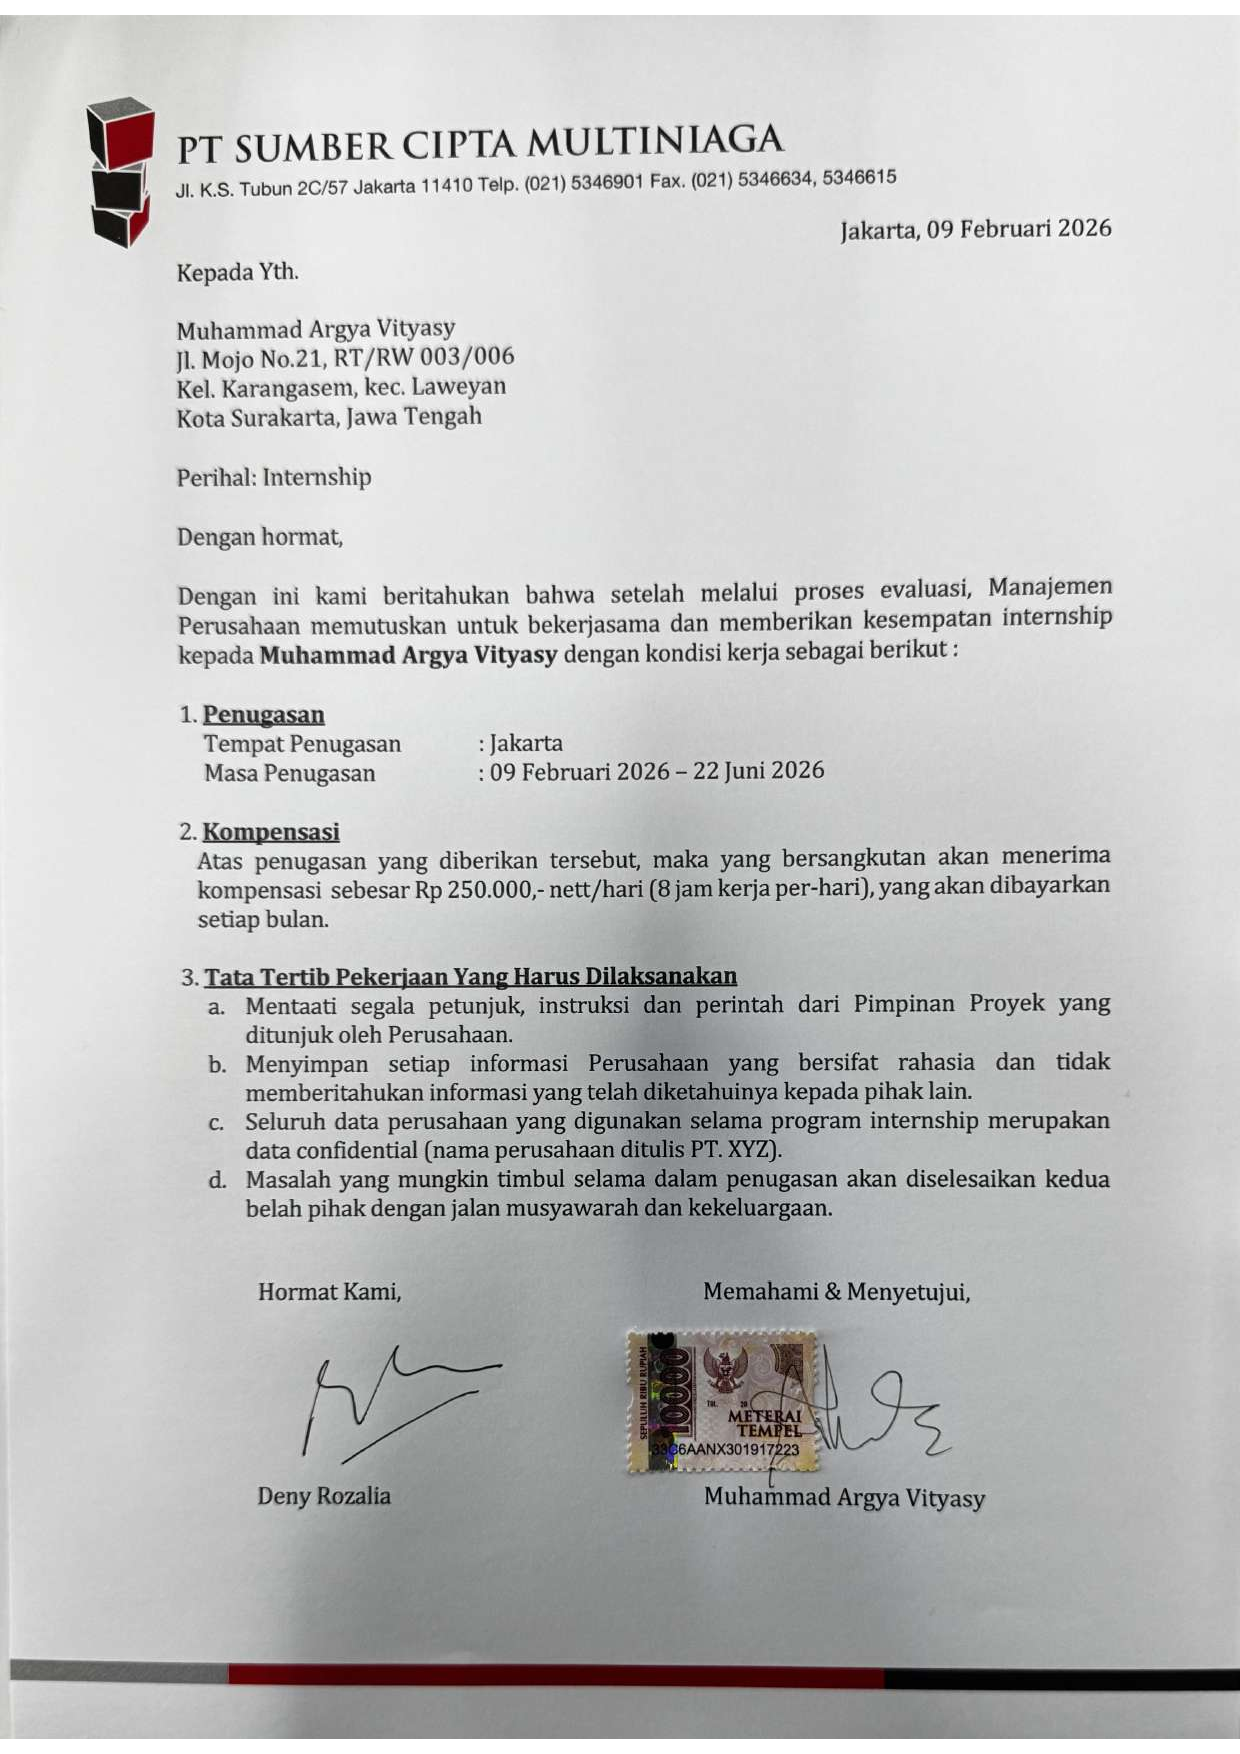
\includegraphics[width=0.9\textwidth]{gambar/loa.pdf} % Replace with actual file
\end{center}

\newpage
\subsection*{ii. Surat Izin Dekan}
\begin{center}
    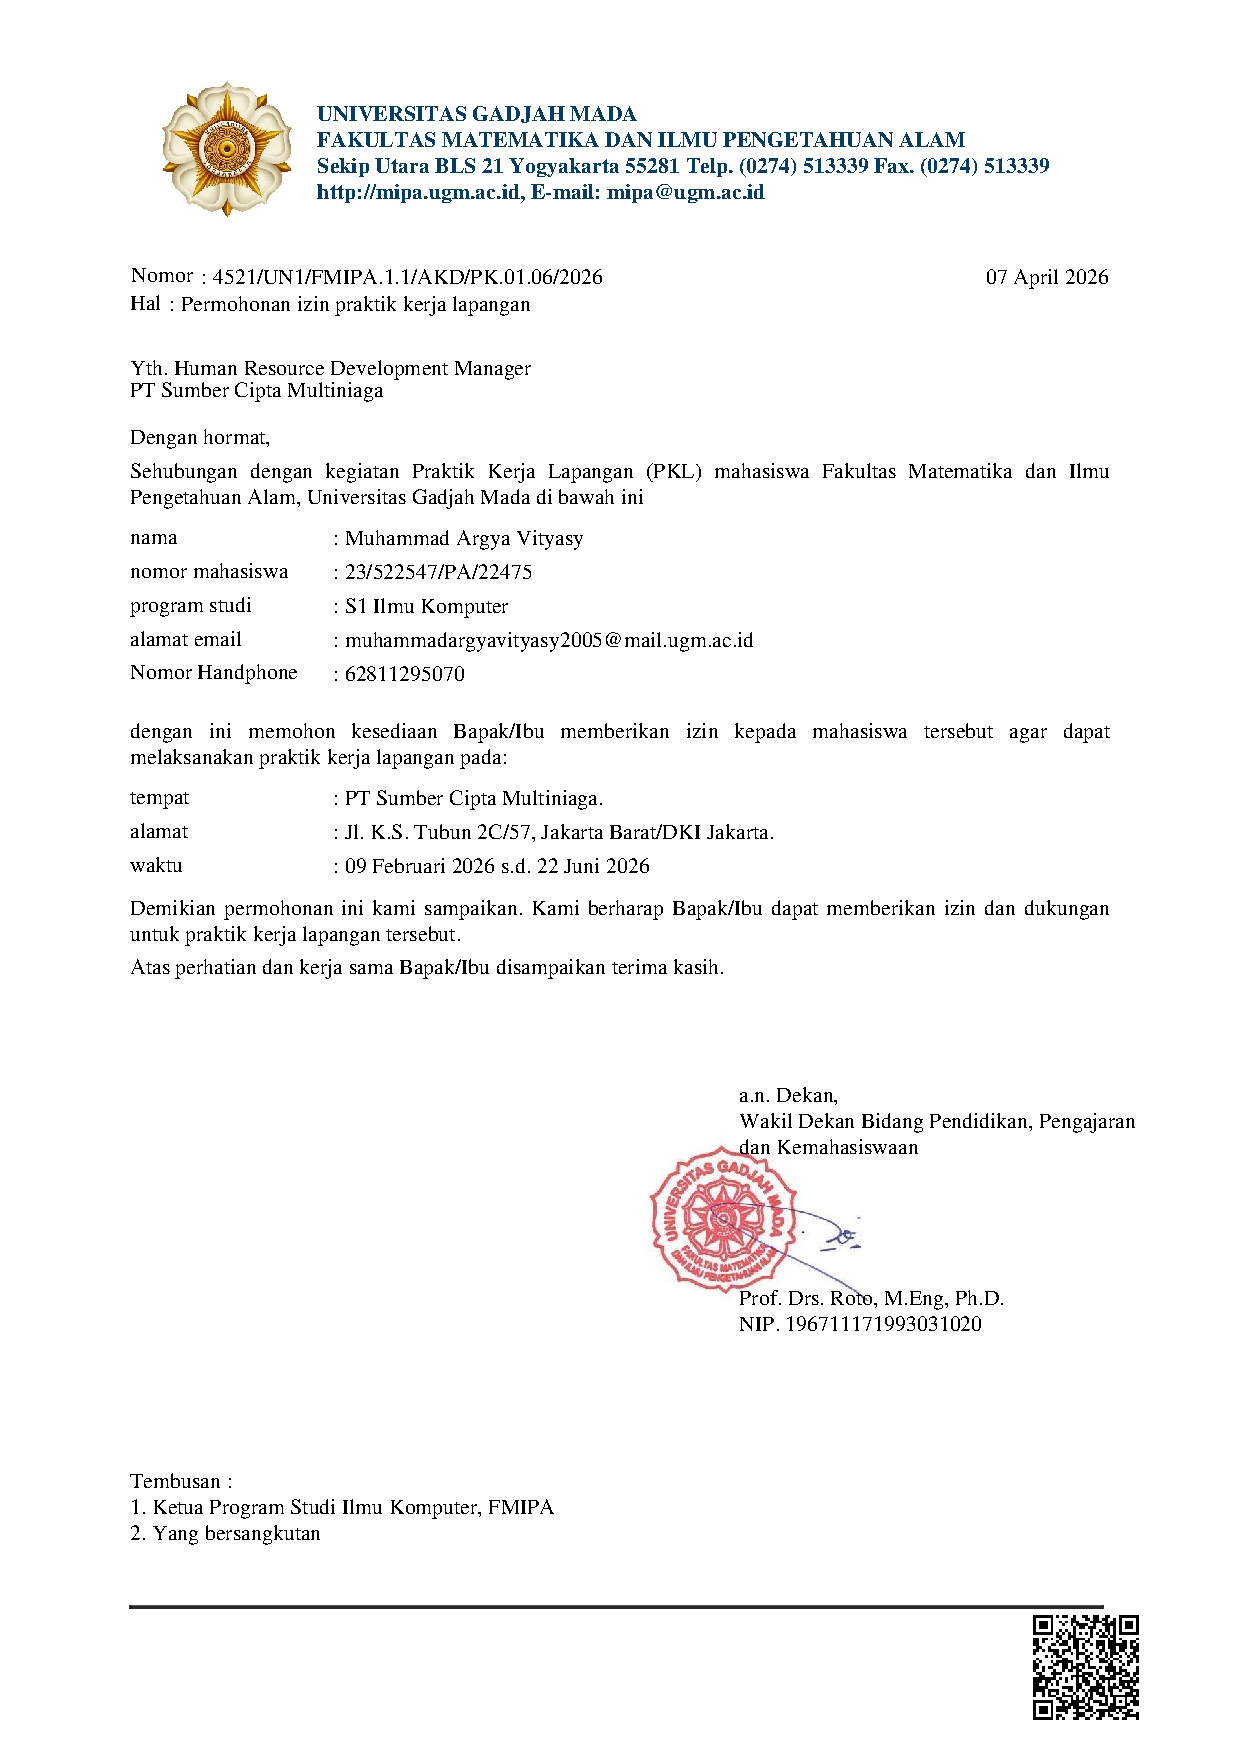
\includegraphics[width=0.9\textwidth]{gambar/surat_izin_dekan.pdf} % Replace with actual file
\end{center}

\newpage
\subsection*{iii. Surat Izin Magang}
\begin{center}
    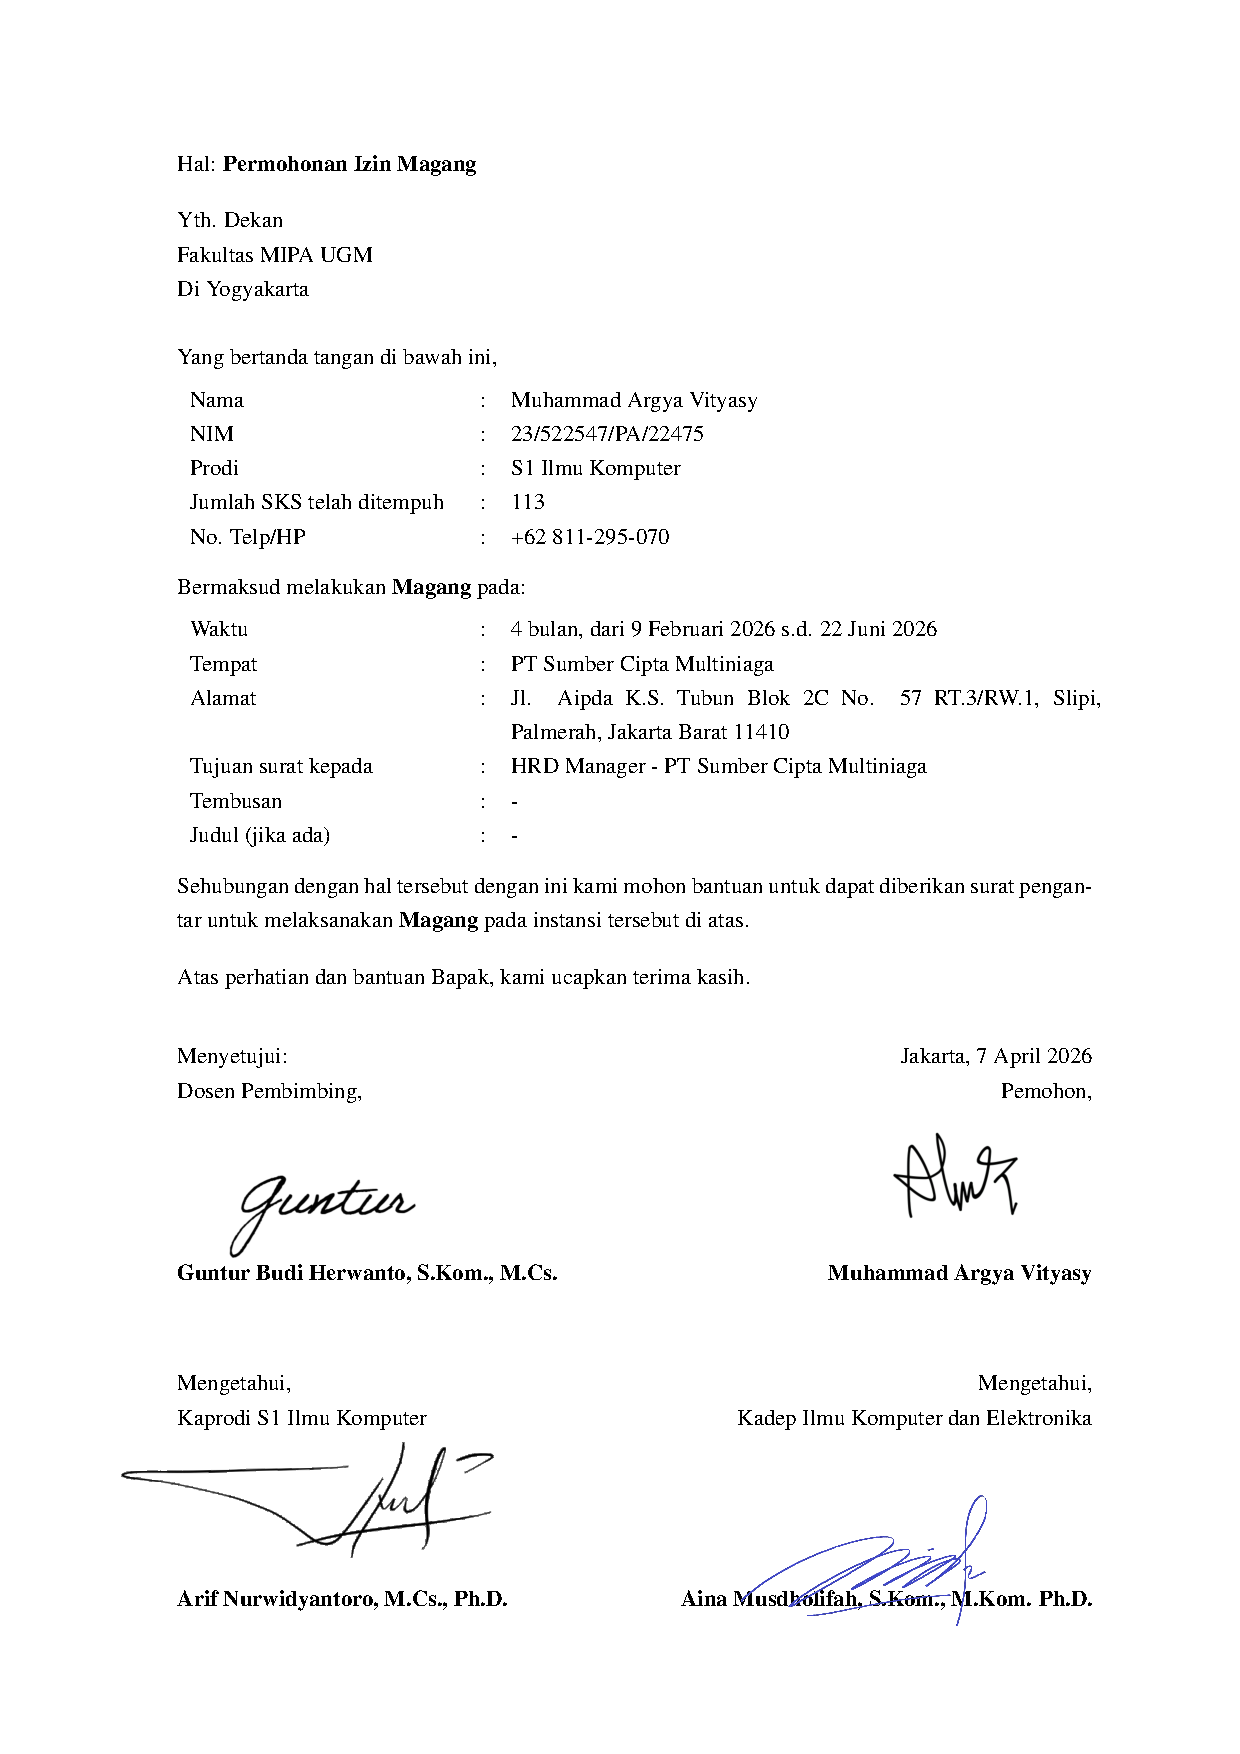
\includegraphics[width=0.9\textwidth]{gambar/surat_izin_magang.pdf} % Replace with actual file
\end{center}

\end{document}